% ============================================================
\chapter{Mesures Sign\'ees et D\'ecomposition de Hahn-Jordan}
\label{ch:mesures_signees}
% ============================================================

\section{Introduction}

Jusqu'\`a pr\'esent, les mesures \'etaient des quantit\'es positives~: surface, volume, probabilit\'e. Mais la physique et l'\'economie regorgent de grandeurs qui changent de signe~: une charge \'electrique peut \^etre positive ou n\'egative, un bilan financier peut \^etre b\'en\'eficiaire ou d\'eficitaire, la diff\'erence de deux mesures de probabilit\'e n'est plus une mesure positive. Johann Radon et Otton Nikodym, dans les ann\'ees 1910--1930, ont montr\'e que toute mesure sign\'ee se d\'ecompose canoniquement en une partie positive et une partie n\'egative (d\'ecomposition de Jordan), concentr\'ees sur des ensembles disjoints (d\'ecomposition de Hahn). Le th\'eor\`eme de Radon--Nikodym, qui exprime une mesure absolument continue par rapport \`a une autre comme une int\'egrale pond\'er\'ee, couronne cette th\'eorie et fournit la d\'efinition rigoureuse de la densit\'e de probabilit\'e.

\begin{intuition}[title=\textbf{Pourquoi des mesures sign\'ees~?}]
Imaginez une distribution de charge \'electrique sur une surface~: certaines r\'egions
portent une charge positive, d'autres une charge n\'egative. La \og mesure de charge \fg
totale d'un ensemble peut \^etre positive, n\'egative ou nulle. C'est exactement ce que
mod\'elise une mesure sign\'ee. De plus, la diff\'erence de deux mesures (positives) finies
est toujours une mesure sign\'ee.
\end{intuition}

% ------------------------------------------------------------
\section{D\'efinitions et premiers exemples}
% ------------------------------------------------------------

\begin{definition}[Mesure sign\'ee]
\label{def:mesure_signee}
Soit $(X, \mathcal{A})$ un espace mesurable. Une \emph{mesure sign\'ee}\index{mesure sign\'ee}
sur $(X, \mathcal{A})$ est une application $\nu : \mathcal{A} \to [-\infty, +\infty]$
v\'erifiant~:
\begin{enumerate}
    \item[(i)] $\nu(\varnothing) = 0$\,;
    \item[(ii)] $\nu$ ne prend \emph{au plus} qu'une des valeurs $+\infty$ et $-\infty$\,;
    \item[(iii)] (\emph{$\sigma$-additivit\'e}) pour toute suite $(A_n)_{n \geq 1}$
    d'\'el\'ements mutuellement disjoints de $\mathcal{A}$~:
    \[
        \nu\!\left(\bigcup_{n=1}^{\infty} A_n\right)
        = \sum_{n=1}^{\infty} \nu(A_n),
    \]
    o\`u la s\'erie converge absolument si le membre de gauche est fini.
\end{enumerate}
\end{definition}

\begin{remarque}
La condition (ii) est essentielle pour \'eviter les expressions ind\'etermin\'ees de la
forme $+\infty - \infty$. Si $\nu$ ne prend pas la valeur $-\infty$ (resp.\ $+\infty$),
on dit que $\nu$ ne prend pas la valeur $-\infty$ par le bas (resp.\ par le haut).
\end{remarque}

\begin{exemple}
\begin{enumerate}
    \item Si $\mu$ et $\lambda$ sont deux mesures positives sur $(X, \mathcal{A})$
    avec $\lambda$ finie, alors $\nu = \mu - \lambda$ est une mesure sign\'ee.
    \item Soit $f \in L^1(\mu)$. L'application
    $\nu(A) = \int_A f\, d\mu$ est une mesure sign\'ee finie.
    \item Toute mesure positive est une mesure sign\'ee (cas particulier).
\end{enumerate}
\end{exemple}

\begin{definition}[Ensemble positif, n\'egatif, nul]
Soit $\nu$ une mesure sign\'ee sur $(X, \mathcal{A})$.
\begin{itemize}
    \item Un ensemble $A \in \mathcal{A}$ est dit \emph{positif}\index{ensemble positif}
    pour $\nu$ si $\nu(B) \geq 0$ pour tout $B \in \mathcal{A}$ avec $B \subset A$.
    \item Un ensemble $A$ est dit \emph{n\'egatif}\index{ensemble n\'egatif}
    pour $\nu$ si $\nu(B) \leq 0$ pour tout $B \in \mathcal{A}$ avec $B \subset A$.
    \item Un ensemble $A$ est dit \emph{nul}\index{ensemble nul} pour $\nu$
    si $\nu(B) = 0$ pour tout $B \in \mathcal{A}$ avec $B \subset A$.
\end{itemize}
\end{definition}

\begin{attention}[title=\textbf{Positif pour $\nu$ $\neq$ $\nu(A) \geq 0$}]
Un ensemble $A$ est positif pour $\nu$ si \emph{tous} ses sous-ensembles mesurables
ont une mesure sign\'ee positive. Le fait que $\nu(A) \geq 0$ ne suffit pas~: il
pourrait exister $B \subset A$ avec $\nu(B) < 0$.
\end{attention}

% ------------------------------------------------------------
\section{D\'ecomposition de Hahn}
% ------------------------------------------------------------

\begin{lemme}
\label{lem:hahn_negatif}
Soit $\nu$ une mesure sign\'ee sur $(X, \mathcal{A})$ et soit $A \in \mathcal{A}$
avec $-\infty < \nu(A) < 0$. Alors il existe un ensemble n\'egatif $B \subset A$
tel que $\nu(B) \leq \nu(A)$.
\end{lemme}

\begin{proof}
Si $A$ est d\'ej\`a n\'egatif, on pose $B = A$. Sinon, il existe $A_1 \subset A$
avec $\nu(A_1) > 0$. Soit $n_1$ le plus petit entier tel qu'il existe
$A_1 \subset A$ mesurable avec $\nu(A_1) \geq 1/n_1$. On it\`ere~: dans
$A \setminus A_1$, si celui-ci n'est pas n\'egatif, on trouve $A_2$ avec
$\nu(A_2) \geq 1/n_2$, etc. Posons $B = A \setminus \bigcup_{k=1}^{\infty} A_k$.
Alors $\nu(B) = \nu(A) - \sum_{k} \nu(A_k) \leq \nu(A) < 0$, et
$\sum_k 1/n_k \leq \nu(A \setminus B) - \nu(A) < \infty$, donc $1/n_k \to 0$.
Si $C \subset B$ v\'erifiait $\nu(C) > 0$, il existerait $n$ avec $\nu(C) \geq 1/n$,
contredisant le choix de $n_k$ \`a l'\'etape $k$ lorsque $1/n_k < 1/n$. Donc $B$ est
n\'egatif.
\end{proof}

% Diagramme de la d\'ecomposition de Hahn
\begin{center}
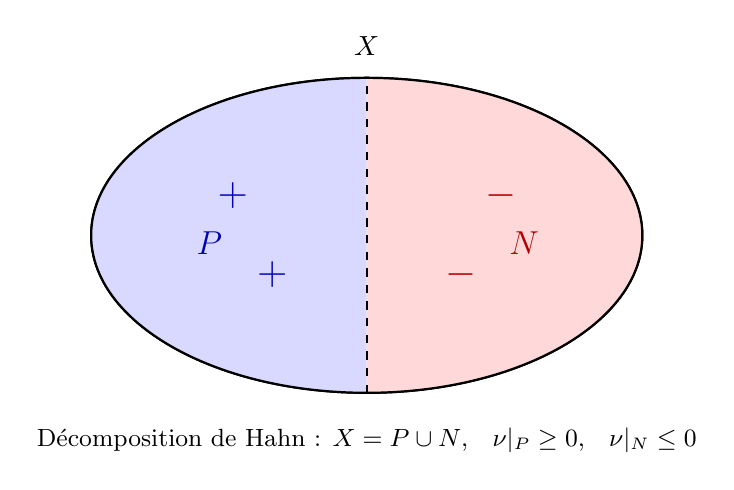
\begin{tikzpicture}[scale=1.0]
  % Ensemble X (ellipse ext\'erieure)
  \draw[thick] (0,0) ellipse (3.5cm and 2cm);
  \node at (0,2.4) {$X$};
  % Ligne de s\'eparation
  \draw[thick, dashed] (0,-2) -- (0,2);
  % R\'egion P (positive, bleu)
  \fill[blue!15] (0,0) -- (0,2) arc[start angle=90, end angle=270,
    x radius=3.5cm, y radius=2cm] -- cycle;
  % R\'egion N (n\'egative, rouge)
  \fill[red!15] (0,0) -- (0,2) arc[start angle=90, end angle=-90,
    x radius=3.5cm, y radius=2cm] -- cycle;
  % Re-tracer le contour et la s\'eparation
  \draw[thick] (0,0) ellipse (3.5cm and 2cm);
  \draw[thick, dashed] (0,-2) -- (0,2);
  % \'Etiquettes et signes
  \node[blue!70!black, font=\Large\bfseries] at (-1.7,0.5) {$+$};
  \node[blue!70!black, font=\Large\bfseries] at (-1.2,-0.5) {$+$};
  \node[red!70!black, font=\Large\bfseries] at (1.7,0.5) {$-$};
  \node[red!70!black, font=\Large\bfseries] at (1.2,-0.5) {$-$};
  \node[blue!70!black, font=\large] at (-2.0,-0.1) {$P$};
  \node[red!70!black, font=\large] at (2.0,-0.1) {$N$};
  % L\'egende
  \node at (0,-2.6) {\small D\'ecomposition de Hahn~: $X = P \cup N$, \;
    $\nu|_P \geq 0$, \; $\nu|_N \leq 0$};
\end{tikzpicture}
\end{center}

\begin{theoreme}[D\'ecomposition de Hahn]
\label{thm:hahn}
\index{d\'ecomposition de Hahn}
Soit $\nu$ une mesure sign\'ee sur $(X, \mathcal{A})$. Il existe une partition
$X = P \cup N$ avec $P, N \in \mathcal{A}$, $P \cap N = \varnothing$, telle que
$P$ est un ensemble positif et $N$ est un ensemble n\'egatif pour $\nu$.

De plus, cette d\'ecomposition est \emph{essentiellement unique}~: si
$X = P' \cup N'$ est une autre d\'ecomposition de Hahn, alors $P \triangle P'$
(et $N \triangle N'$) est un ensemble nul pour $\nu$.
\end{theoreme}

\begin{proof}
Supposons que $\nu$ ne prend pas la valeur $+\infty$ (le cas sym\'etrique est analogue).
Posons $\lambda = \inf\{\nu(A) : A \in \mathcal{A}\} \in [-\infty, 0]$. Pour chaque
$n \geq 1$, il existe $A_n \in \mathcal{A}$ avec $\nu(A_n) < \lambda + 1/n$. Par
le lemme~\ref{lem:hahn_negatif}, il existe un ensemble n\'egatif $B_n \subset A_n$
avec $\nu(B_n) \leq \nu(A_n) < \lambda + 1/n$.

Posons $N = \bigcup_{n=1}^{\infty} B_n$. Comme r\'eunion d\'enombrable d'ensembles
n\'egatifs, $N$ est n\'egatif. De plus, $\nu(N) \leq \nu(B_n) < \lambda + 1/n$ pour
tout $n$, donc $\nu(N) = \lambda > -\infty$ (car $\nu$ ne prend pas la valeur $-\infty$
par hypoth\`ese, puisqu'elle ne prend pas $+\infty$, c'est $-\infty$ qui est \'eventuellement
exclue --- en fait $\lambda > -\infty$ car $\nu(N)$ est fini ou \'egal \`a $\lambda$).

Posons $P = X \setminus N$. Si $P$ n'\'etait pas positif, il existerait $A \subset P$
avec $\nu(A) < 0$, d'o\`u un ensemble n\'egatif $B \subset A$ avec $\nu(B) \leq \nu(A) < 0$.
Mais alors $N \cup B$ serait n\'egatif avec $\nu(N \cup B) = \nu(N) + \nu(B) < \nu(N)$,
contredisant la d\'efinition de $\lambda$.

Pour l'unicit\'e essentielle~: si $X = P' \cup N'$ est une autre d\'ecomposition, alors
$P \cap N' \subset P$ (positif) et $P \cap N' \subset N'$ (n\'egatif), donc $P \cap N'$
est nul. De m\^eme $P' \cap N$ est nul, et $P \triangle P' \subset (P \cap N') \cup (P' \cap N)$.
\end{proof}

% ------------------------------------------------------------
\section{D\'ecomposition de Jordan et variation totale}
% ------------------------------------------------------------

\begin{definition}[D\'ecomposition de Jordan]
\label{def:jordan}
\index{d\'ecomposition de Jordan}
Soit $\nu$ une mesure sign\'ee sur $(X, \mathcal{A})$ et $X = P \cup N$ une
d\'ecomposition de Hahn. On d\'efinit les \emph{parties positive et n\'egative} de
$\nu$ par~:
\[
    \nu^+(A) = \nu(A \cap P), \qquad \nu^-(A) = -\nu(A \cap N),
\]
pour tout $A \in \mathcal{A}$. On a alors $\nu = \nu^+ - \nu^-$.
\end{definition}

\begin{theoreme}[D\'ecomposition de Jordan]
Les mesures $\nu^+$ et $\nu^-$ sont des mesures positives sur $(X, \mathcal{A})$,
au moins l'une des deux est finie, et elles ne d\'ependent pas du choix de la
d\'ecomposition de Hahn (elles sont uniquement d\'etermin\'ees par $\nu$).

De plus, $\nu = \nu^+ - \nu^-$ et $\nu^+ \perp \nu^-$ (les mesures $\nu^+$ et
$\nu^-$ sont mutuellement singuli\`eres).
\end{theoreme}

\begin{proof}
La positivit\'e de $\nu^+$ et $\nu^-$ d\'ecoule du fait que $P$ est positif et $N$
est n\'egatif. La $\sigma$-additivit\'e est imm\'ediate. Comme $\nu$ ne prend au plus
qu'une valeur infinie, au moins l'une de $\nu^+$, $\nu^-$ est finie. L'ind\'ependance
vis-\`a-vis du choix de la d\'ecomposition r\'esulte de l'unicit\'e essentielle.
La singularit\'e mutuelle vient de $\nu^+(N) = 0$ et $\nu^-(P) = 0$.
\end{proof}

\begin{definition}[Variation totale]
\label{def:variation_totale}
\index{variation totale}
La \emph{variation totale} de $\nu$ est la mesure positive~:
\[
    \abs{\nu} = \nu^+ + \nu^-.
\]
La \emph{variation totale de $\nu$ sur $X$} est le nombre
$\norm{\nu} = \abs{\nu}(X) = \nu^+(X) + \nu^-(X)$.
\end{definition}

\begin{proposition}[Propri\'et\'es de la variation totale]
Pour toute mesure sign\'ee $\nu$ et tout $A \in \mathcal{A}$~:
\begin{enumerate}
    \item $\abs{\nu(A)} \leq \abs{\nu}(A)$\,;
    \item $\abs{\nu}(A) = \sup\left\{\sum_{i=1}^n \abs{\nu(A_i)} :
    A = \bigsqcup_{i=1}^n A_i,\, A_i \in \mathcal{A}\right\}$\,;
    \item $\nu$ est une mesure sign\'ee finie si et seulement si
    $\abs{\nu}(X) < \infty$.
\end{enumerate}
\end{proposition}

\begin{proof}
(1) $\abs{\nu(A)} = \abs{\nu^+(A) - \nu^-(A)} \leq \nu^+(A) + \nu^-(A) = \abs{\nu}(A)$.

(2) Soit $A = \bigsqcup_{i=1}^n A_i$. Alors
$\sum_i \abs{\nu(A_i)} \leq \sum_i \abs{\nu}(A_i) = \abs{\nu}(A)$, d'o\`u
$\sup \leq \abs{\nu}(A)$. Pour l'in\'egalit\'e inverse, prendre la partition
$A = (A \cap P) \sqcup (A \cap N)$ donne
$\nu^+(A) + \nu^-(A) = \abs{\nu(A \cap P)} + \abs{\nu(A \cap N)}$.

(3) Imm\'ediat car $\norm{\nu} = \nu^+(X) + \nu^-(X)$.
\end{proof}

\begin{formules}[title=\textbf{R\'esum\'e~: d\'ecomposition de Jordan}]
Pour toute mesure sign\'ee $\nu$~:
\begin{align*}
    \nu &= \nu^+ - \nu^-, \qquad \abs{\nu} = \nu^+ + \nu^-, \\
    \nu^+ &= \frac{\abs{\nu} + \nu}{2}, \qquad
    \nu^- = \frac{\abs{\nu} - \nu}{2}.
\end{align*}
\end{formules}

% ------------------------------------------------------------
\section{Singularit\'e mutuelle}
% ------------------------------------------------------------

\begin{definition}[Mesures mutuellement singuli\`eres]
\label{def:singuliere}
\index{mesures mutuellement singuli\`eres}
Deux mesures sign\'ees $\mu$ et $\nu$ sur $(X, \mathcal{A})$ sont dites
\emph{mutuellement singuli\`eres}\index{singularit\'e mutuelle}, not\'e
$\mu \perp \nu$, s'il existe une partition $X = A \cup B$ avec
$A, B \in \mathcal{A}$ telle que $\abs{\mu}(B) = 0$ et $\abs{\nu}(A) = 0$.
\end{definition}

\begin{exemple}
\begin{enumerate}
    \item La mesure de Lebesgue $\lambda$ sur $\R$ et la mesure de Dirac
    $\delta_0$ sont mutuellement singuli\`eres~: $\lambda(\{0\}) = 0$ et
    $\delta_0(\R \setminus \{0\}) = 0$.
    \item La mesure de Lebesgue et la mesure de Cantor--Vitali sur $[0,1]$
    sont mutuellement singuli\`eres.
\end{enumerate}
\end{exemple}

\begin{proposition}
La relation $\perp$ est sym\'etrique. Si $\mu \perp \nu$ et $\mu \perp \lambda$,
alors $\mu \perp (\nu + \lambda)$ (lorsque la somme est d\'efinie).
\end{proposition}

% ------------------------------------------------------------
\section{Espace des mesures sign\'ees finies}
% ------------------------------------------------------------

\begin{proposition}
L'ensemble $\mathcal{M}(X, \mathcal{A})$ des mesures sign\'ees finies sur
$(X, \mathcal{A})$ est un espace vectoriel r\'eel, et
$\norm{\nu} = \abs{\nu}(X)$ est une norme sur cet espace. De plus,
$(\mathcal{M}(X, \mathcal{A}), \norm{\cdot})$ est un espace de Banach.
\end{proposition}

% ------------------------------------------------------------
\section{Exercices}
% ------------------------------------------------------------

\begin{exercice}
Soit $\nu$ une mesure sign\'ee finie sur $(X, \mathcal{A})$. Montrer que $\nu$
est born\'ee, c'est-\`a-dire $\sup_{A \in \mathcal{A}} \abs{\nu(A)} < \infty$.
\end{exercice}

\begin{exercice}
Soit $f \in L^1(\R, \lambda)$ o\`u $\lambda$ est la mesure de Lebesgue. Montrer
que $\nu(A) = \int_A f\, d\lambda$ d\'efinit une mesure sign\'ee et calculer
$\nu^+$, $\nu^-$ et $\abs{\nu}$ en fonction de $f$.
\emph{Indication}~: montrer que $\nu^+(A) = \int_A f^+\, d\lambda$ et
$\nu^-(A) = \int_A f^-\, d\lambda$.
\end{exercice}

\begin{exercice}
Montrer que deux mesures positives $\mu$ et $\nu$ sont mutuellement singuli\`eres
si et seulement si $\inf_{A \in \mathcal{A}} [\mu(A) + \nu(A^c)] = 0$.
\end{exercice}

\begin{exercice}
Soit $\nu$ une mesure sign\'ee et $(A_n)$ une suite croissante dans $\mathcal{A}$.
Montrer que $\nu(\bigcup_n A_n) = \lim_n \nu(A_n)$ (continuit\'e monotone
pour les mesures sign\'ees).
\end{exercice}

\begin{exercice}[D\'ecomposition de Hahn explicite]
Soit $\nu$ la mesure sign\'ee sur $(\R, \mathcal{B}(\R))$ d\'efinie par
$\nu(A) = \int_A (x^2 - 1) e^{-x^2}\, d\lambda(x)$. D\'eterminer une
d\'ecomposition de Hahn de $\R$ pour $\nu$ et en d\'eduire $\nu^+$, $\nu^-$.
\end{exercice}

\begin{exercice}
Soit $\nu$ une mesure sign\'ee finie. Montrer que pour tout $\varepsilon > 0$,
l'ensemble $\{A \in \mathcal{A} : \abs{\nu(A)} > \varepsilon\}$ est fini.
\emph{Indication}~: utiliser $\abs{\nu}(X) < \infty$.
\end{exercice}
